\documentclass[11pt]{article}
\usepackage{deauthor}
\usepackage{times}
\usepackage{graphicx}
\usepackage{xspace}
%\usepackage{xcolor}
\usepackage[square,numbers]{natbib}
\usepackage[table,xcdraw]{xcolor}

\newenvironment{denselist}{
    \begin{list}{\small{$\bullet$}}%
    {\setlength{\itemsep}{0ex} \setlength{\topsep}{0ex}
    \setlength{\parsep}{0pt} \setlength{\itemindent}{0pt}
    \setlength{\leftmargin}{1.5em}
    \setlength{\partopsep}{0pt}}}%
    {\end{list}}

\newcommand{\squishlist}{
   \begin{list}{$\bullet$}
    { \setlength{\itemsep}{0pt}
      \setlength{\parsep}{2pt}
      \setlength{\topsep}{0pt}
      \setlength{\partopsep}{0pt}
      \leftmargin=25pt
\rightmargin=0pt
\labelsep=5pt
\labelwidth=10pt
\itemindent=0pt
\listparindent=0pt
\itemsep=\parsep
    }
}
\newcommand{\squishend}{\end{list}}

\setlength{\parindent}{0cm}
\setlength{\parskip}{2pt}
% use extensively to toggle between paper and TR
\newcommand{\eat}[1]{}
% \newcommand{\papertext}[1]{{\leavevmode\color{blue}{#1}}}
% \newcommand{\techreport}[1]{{\leavevmode\color{red}{#1}}}
\newcommand{\papertext}[1]{#1}
\newcommand{\techreport}[1]{}
\newcommand{\boldpara}[1]{\textbf{\paragraph{#1}}}
% de-facto paragraph format
\newcommand{\stitle}[1]{\par\noindent\textbf{#1}}
\newcommand{\tvcg}[1]{{\leavevmode\color{blue}{#1}}}
\newcommand{\cut}[1]{{\leavevmode\color{lightgray}{#1}}}
\newcommand{\ccut}[1]{} %confirmed cut
\def\plainauthor{Doris Jung-Lin Lee, Aditya Parameswaran}
\def\emptyauthor{} 
\def\plainkeywords{Data visualization, exploratory data analysis, visual querying.}
\def\plaingeneralterms{Documentation, Standardization}

\newcommand{\zv}{\textit{zenvisage}\xspace}
\newcommand{\vida}{\textsc{VIDA}\xspace}
\newcommand{\sbd}{\textsc{Storyboard}\xspace}
\newcommand{\seedb}{\textsc{SeeDB}\xspace}
\newcommand{\agp}[1]{\textcolor{green}{Aditya: #1}}
\newcommand{\dor}[1]{\textcolor{blue}{Doris: #1}} 

\newcommand\notes[1]{\textcolor{red}{#1}}

% To make various LaTeX processors do the right thing with page size.
\def\pprw{8.5in}
\def\pprh{11in}
\special{papersize=\pprw,\pprh}
\setlength{\paperwidth}{\pprw}
\setlength{\paperheight}{\pprh}
\setlength{\pdfpagewidth}{\pprw}
\setlength{\pdfpageheight}{\pprh}
%%%%%%%%%%%%%%%%%%%%%%%%%%%%%%%%%%%%%%%%%%%%

\begin{document}
% \title{Towards a Visual Discovery Assistant: The New Frontier in Accelerating Visual Data Exploration}
% \title{Towards Automating Visual Data Exploration with \\ a Visual Discovery Assistant}
% \title{The Case for a Visual Discovery Assistant: \\ Challenges and Opportunities}
\title{The Case for a {\em Visual Discovery Assistant}: \\ A Holistic Solution for Accelerating Visual Data Exploration}
%\title{From Search to Recommendation: Towards Visual Discovery Assistant}
% \title{Navigating Visualization Collections}
%\title{Towards a Holistic Workflow for Visual Data Exploration}
\author{\plainauthor\\
\{jlee782,adityagp\}@illinois.edu\\
University of Illinois, Urbana-Champaign}
\maketitle
\begin{abstract}
Visualization is one of the 
most effective and widely-used 
techniques for understanding data. 
Yet, the growing use of visualizations 
for exploratory data analysis 
presses new demands beyond simply 
the graphical presentation 
and visualization authoring 
capabilities offered in existing tools. 
In particular, many data analysis
tasks involve navigating large 
collections of visualizations to make sense
of trends in data;
at present, this navigation is done manually or
programmatically. 
We outline a vision for an
intelligent, interactive, understandable,
and usable tool 
that can help automate
this largely manual navigation: we call our tool \vida\footnote{Vida is short for {\em life} in Spanish.}---short for {VIsual Discovery Assistant}. 
We argue that typical navigation tasks can be 
organized across two dimensions---overall goal 
and precision of specification.
We organize prior work---both our own work, as well
as other ongoing work in this area---across 
these two dimensions, and highlight
new research challenges.
Together, addressing these challenges underlying \vida
can help pave the way for a comprehensive
solution for removing the pain points
in visual data exploration.
% We outline a vision for a new breed of 
% interactive tools that can help automate
% this largely manual navigation process. 
% We argue that these tools need to span two 
% dimensions---precision and task.
% We organize prior work---both our own work, as well
% as other ongoing work in this area---to highlight
% new research challenges
% across these two dimensions.
% Together, addressing these challenges
% can help provide a comprehensive solution 
% for navigating and making sense of 
% large collections of visualizations. 
% In this paper, we describe three areas of visual data exploration facing these challenges. First, we introduce the problem of precise querying: how to search for a desired trend or pattern given the large space of visualizations that could be generate from a given dataset. As vague and complex queries cannot often be addressed through interactions in precise visual querying systems, we introduce a class of intelligent visual querying systems that allows users provide feedback in order to clarify and refine their queries. Finally, even with a omnipotent system that addresses any given visual query, users may not know what to query. Therefore, we advocate for recommendations that facillitates distributional and contextual awareness to help users gain more holistic data understanding, guide them towards meaningful insights, and jumpstart further inquiries. We describe the exemplary systems drawing from both our own work (\zv and \sbd) and ongoing research in the area to highlight future directions and opportunties in this space.
% This paper surveys the emerging field of formally reasoning
% about and optimizing open-ended crowdsourcing, a popular and crucially important, but severely
% understudied class of crowdsourcing—the next frontier in crowdsourced data management. The underlying
% challenges include distilling the right answer when none of the workers agree with each other,
% teasing apart the various perspectives adopted by workers when answering tasks, and effectively selecting
% between the many open-ended operators appropriate for a problem. We describe the approaches that
% we’ve found to be effective for open-ended crowdsourcing, drawing from our experiences in this space.
\end{abstract}

% Eventually, we need to compile all of these into one single file  during submission time. 
%!TEX root = main.tex
\section{Introduction}% 

\par 
With the ever-increasing complexity 
and size of datasets,
there is a growing demand for 
information visualization tools
that can help data scientists make sense of large
volumes of data.
Visualizations help discover 
trends and patterns, 
spot outliers and anomalies, 
and generate or verify hypotheses.
Moreover, 
visualizations are visceral and intuitive: 
they tell us stories about our data; 
they educate, delight, inform, 
enthrall, amaze, and clarify.
This has led to the overwhelming popularity
of point-and-click visualization tools like Tableau~\cite{Stolte2002},
as well as programmatic toolkits like ggplot, D3, Vega, and matplotlib. 
We term these tools as {\em visualization-at-a-time} approaches, since
data scientists need to individually 
generate each visualization (via code or interactions),
and examine them, 
one at a time.


\par
As datasets grow in size and complexity, 
these visualization-at-a-time approaches start to break down,
due to the limited time availability on the 
part of the data scientists---there 
are often too many visualizations to examine for a given 
task, such as identifying outliers, or inferring patterns. 
Even on a single table, 
visualizations can be generated
by varying the subsets of data operated on, 
or the attributes (or combinations
thereof) that can be visualized. 
If we add in various visualization modalities, encodings,
aesthetics, binning methods, and transformations,
this space becomes even larger.


\par
Thus, there is a pressing need for an 
intelligent,
interactive, understandable, usable, and
enjoyable tool that can help 
data scientists navigate
collections of visualizations.
We term our hypothesized tool \vida,
short for {\em VIsual Discovery Assistant}.
Data scientists specify their discovery
goal at a high level,
with \vida 
automatically 
traversing visualizations to provide
solutions or partial solutions for the
specified discovery goal, thereby
eliminating the tedium and wasted
labor of comparable visualization-at-a-time 
approaches.

\par
\stitle{\vida Dimensions.} In order to be a holistic solution for 
navigating collections of visualizations,
\vida must be able to support various discovery
settings. 
We organize these settings along two
dimensions, displayed along the columns and 
rows (respectively) of Table~\ref{fig:table}---first, the overall discovery goal,
and second, the degree of specificity of the goal.
We also cite references (described later on)
for systems that partially provide the necessary
functionality for the given setting.
We call these systems Visual Querying Systems, or VQSs for short.


\begin{wrapfigure}{l}{0.5\textwidth}
\centering
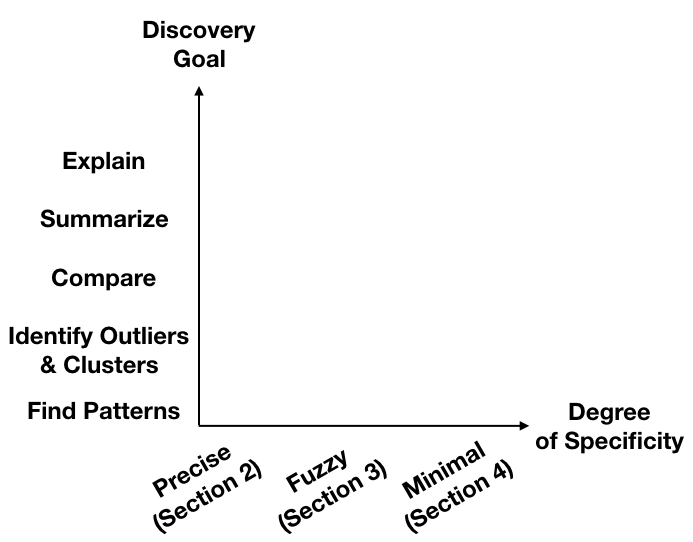
\includegraphics[width=\linewidth]{figures/dimensions_cropped.png}
\vspace{-10pt}
\caption{Dimensions of VQSs. Columns are organized into discovery goals and rows are ordered by decreasing levels of query specificity and correspondingly increasing levels of autonomous assistance.}\label{fig:table}
\vspace{-15pt}
\end{wrapfigure}

\par
 We identify five 
common discovery goals in visual data exploration, organized
along the columns:
{\em finding patterns}, {\em identifying anomalies/clusters}, {\em summarizing}, 
{\em performing comparisons}, {\em providing explanations}.
These five goals borrow borrow from functionalities in existing
systems, as well as related visualization task taxonomies~\cite{Heer2012,Amar2005}.
We omit low-level goals such as filtering or sorting, since
these functionalities are common in 
visualization-at-a-time tools and toolkits.
We also omit goals that go beyond visual data exploration,
such as extrapolation, supervised learning, and cleaning, among others. 

\par 
 We identify three degrees of specificity
for the discovery goal, organized along the rows:
{\em precise}, {\em fuzzy}, {\em underspecified}.
The degree of specificity characterizes the division
of work between how much user has to specify
versus how much the system has to automatically
infer and aid in accomplishing the discovery goal. 
At the topmost row, the onus is placed on the user
to provide an exact and complete specification of 
what the solution to their discovery
goal must look like;
at the middle row, the user can provide
a vague specification of what the solution must look like;
and finally, at the bottom row,
the user provides a minimal specification, or
leaves the characteristics of the solution underspecified,
leaving it up to the system to ``fill in'' the rest.
Naturally, as we proceed down the rows,
it gets harder for the system to automatically
interpret what the user might have in mind as a solution
to their discovery goal.

\begin{table}[!t]
\scriptsize
\centering
\begin{tabular}{l|l|l|l|l|l}
& \multicolumn{5}{c}{Discovery Goals}                                                                     \\ \hline
& Find Patterns & Identify Anomalies and Clusters      & Compare           & Summarize  & Explain          \\ \hline
Precise (Section~\ref{sec:precise}) & \multicolumn{3}{c|}{Zenvisage~\cite{Lee2017}, ZQL~\cite{Siddiqui2016}}                                      &            &                  \\ \hline
Fuzzy (Section~\ref{sec:vague})     & ShapeSearch\cite{Siddiqui2018}   & Scorpion\cite{Wu2013}, Profiler~\cite{Kandel2012}, Natural Language & Natural Language~\cite{Fast2018,Setlur2016,Hoque2017}  &            & Natural Language \\ \hline
Minimal (Section~\ref{sec:minimal}) &               & \multicolumn{1}{c|}{Storyboard~\cite{Lee2018}}      & SeeDB~\cite{Vartak2015}, Storyboard & Storyboard & Storyboard      
\end{tabular}
\caption{Overview of the systems described in this paper. Columns are organized into discovery goals and rows are ordered by decreasing levels of query specificity and correspondingly increasing levels of autonomous assistance.\agp{fix this. add specificity, augment references}}\label{fig:table}
\end{table}




\par
\stitle{\vida Input Modalities.} To support the spectrum of 
demands imposed by the
discovery settings described above, \vida 
must support a range of interactive input modalities,
as displayed in Figure~\ref{fig:vida_architecture},
catering to a range of user expertise and preferences.
These input modalities include 
\squishlist
	\item natural language, via a keyword search box, or a dialog or conversational interface;
	\item interactions, either with an existing visualization, such as brushing-and-linking or hovering, or those that construct a new one, such as drag-and-drop or sketching; and
	\item restricted template queries, involving selection of operations and operands from a drop-down menu.
\squishend
We will provide examples of these input modalities in subsequent sections.
Each of these inputs are compiled down
into a query in a query language, called \vidaql.
Alternatively, expert users may directly invoke \vidaql queries.
\vidaql queries will natively support the five discovery goals,
and will also support combinations thereof, e.g., pattern search followed by 
summarization. 
Another important element is how much does a user actively ``request'' (pull)
versus \vida ``recommending'' visualizations (push). 
Given that we expect \vida to support a range of specificities,
\vida must support both push and pull, with pull decreasing
in importance, and push rising in importance, as we go from precise to minimal.

\begin{wrapfigure}{r}{0.5\textwidth}
\centering
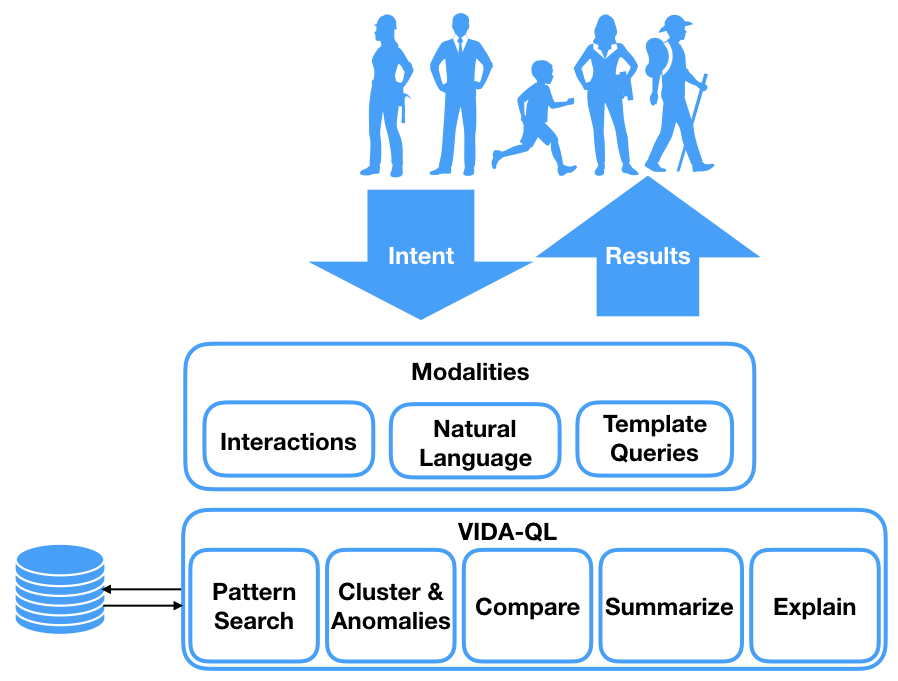
\includegraphics[width=\linewidth]{figures/VIDA_architecture.png}
\vspace{-10pt}
\caption{\vida Architecture\label{fig:vida_architecture}
\vspace{-15pt}
}
\end{wrapfigure}

% \begin{wrapfigure}{r}{0.5\textwidth}
%   \begin{center}
%     \includegraphics[width=0.48\textwidth]{birds}
%   \end{center}
%   \caption{Birds}
% \end{wrapfigure}



% Common framework and module means there are underlying functionalities can be shared (e.g. statistical modules, data heavy-lifting operations)
% - From the top: many different types of users (novices/experts), each with some high-level intent in one of the following modalities:
%      - Interaction: produces as an output either through the creation a visualization (e.g. sketching, drag-and-drop) or changes upon a visualization (e.g. brushing, selections, clicks)
%      - Partial specification includes some minimal input such as input X,Y of interest
%      - Either that or user can directly specify their query exactly in VIDA-QL
% - VIDA-QL contains 5 discovery modules which each have their own "push and pull" components, i.e. work with both search and recommend.

\par
\stitle{Outline.}
The rest of our paper is organized along the degree of specificity
of discovery goal, and we will allude to the specific discovery
goals as well as input modalities as we go along. 
The degree of specificity of the discovery goal is the factor
that most significantly affects the architecture of \vida,
with the complexity increasing as the specificity decreases. 

\par We begin by discussing the 
the {\em precise} setting (Section~\ref{sec:precise}).
We describe \zv~\cite{Siddiqui2016} 
as an example of a solution for
this setting, and thereby a starting point for \vida,
partially eliminating the problem
of having to manually examine large numbers 
of visualizations for a given discovery goal, 
which can be error-prone and inefficient.


\par However, a design study using \zv demonstrates
that the precise setting is insufficient for
addressing all of the demands of real-world use-cases~\cite{Lee2017}.
In particular, users do not have
a clear understanding of their intent or specification 
without looking
at example visualizations or summaries of the data,
and at the same time, their intent or specification is
often not expressible clearly, requiring 
vague or fuzzy high-level notions.

To bridge the gap between the user's high-level
intent and the system demands,
we outline a set of research challenges
that goes beyond simple precise visual querying, by
(a) supporting a wider class of vague or ``high-level''
queries, thereby increasing the expressiveness
of \vida (Section~\ref{sec:vague});
and 
(b) making it easier to know what to query
by recommending visualizations that provide
a high-level understanding of the data (Section~\ref{sec:minimal}).

\agp{We should clarify somewhere that most of our concern is going to 
be the interfaces or query languages, as opposed to optimization,
leveraging parallelism, MQO, sampling, pruning,
which has seen some work --- ZQL, SeeDB, ...}

% In addition, we find that users often do not have a good idea of what they want to query for without looking at example visualizations or summaries of the data. To bridge the gap between user's high-level intent and what the system operates as inputs, we advocate that future research needs to look beyond simple precise visual querying by : 1) making visual query system more expressive by supporting a wider class of vague queries (Section~\ref{sec:vague}) and 2) making it easier to know what to query by recommending visualizations that facilitate data awareness (Section~\ref{sec:minimal}).
% \par Accordingly, the next row in the table highlights a growing class of \textit{intelligent visual querying system} (IVQS) that interprets the `vagueness' of queries and allow users to tweak or refine their queries through a feedback mechanism. \dor{I think we need to expand this definition depending on the new content that we will be adding, ShapeSearch, SeeDB, Scorpion?} 
% \par To address the problem of guiding users to portions of the data that they might be interested in querying, Section~\ref{sec:minimal} introduces systems that help users become more aware of their dataset and visualize where they are in their analysis workflow. The challenge in building these systems involves understanding what types of visualizations should be recommended to facilitate data awareness. As an example, we describe our work on \sbd, a system that provides data summaries and guides users through informative subsets of data. Finally, we discuss related works on how visualizing provenance and situational information can guide users towards more informative analysis actions.
%!TEX root = main.tex
\section{Precise Visual Querying\label{sec:precise}}
Visual analysis often reveal important anomalies or trends in the data\cite{Morton2014}. However, it is often challenging to find the appropriate piece of information to realize these insights.

\subsection{Motivating Example}
Astronomers from the The Dark Energy Survey (DES)\cite{Drlica-Wagner2017} are interested in finding anomalous time series to discover astrophysical transients (objects whose brightness changes dramatically as a function of time), such as supernova explosions or quasars. When trying to find celestial objects corresponding to supernovae, which have a specific pattern of brightness over time, scientists need to individually inspect the visualizations of each object until they find ones that match the pattern. With more than 400 million objects in their catalog, each having their own set of time series brightness measurement, the process of manually exploring a large number of visualizations is not only error-prone, but also overwhelming for scientists who do not have extensive knowledge about their dataset.  
% Intention driven task-based querying (Precise search)
\par The astronomy use case highlights a common challenge in exploratory data analysis (EDA). There is often a large space of possible visualizations that could be generated from a given dataset and manual search through this large collection is inefficient. Visualization authoring tools such as Tableau and Excel focusses on presenting one visualization at a time. There is no systematic way to create, compare, and query large collections of visualizations. 
%\par There has been many related work in this space varying different dimensions of possible visualizations, including visual encodings~\cite{showme}, data facets, . We will focus on  
\subsection{Effortless Data Exploration with \zv}
\par The challenges presented earlier points to a need for tools that enables users to create and search through large collections of visualizations. Therefore, we developed \zv a visual query system that allowed users to search through large collections of visualizations. \zv is built on top of a querying language called ZQL, which provides a mechanism for managing collections of visualizations\cite{Siddiqui}. Contrary prior work on visualization languages for specifying visual encodings of individual visualizations~\cite{Stolte2002,Wilkinson2005}, ZQL supports high-level queries over visualization collections, such as composing, sorting, filtering a collection of visualization. ZQL functionals and primitives can be constructed into rich and expressive query semantics, with functionalties including : 
\begin{itemize}
	\item Finding top-k visualizations whose y values are most or least similar from a queried visualization (e.g. Find other cities with sold price over time similar to Manhattan. Varying along \textsc{city} while keeping \textsc{x=time,y=AVG(price)} fixed.) 
	\item Comparing across a collection of visualizations by iterating over one or more x, y, z attributes while fixing other attributes (e.g. Find a y attribute that varies with time similarly how average price changes over time)
	\item Finding a pair of X and Y axes where two specific visualization instances differ the most. (e.g. For what pair of attributes does the products `stapler' and `chair' differ the most?)
\end{itemize}
\par Given a ZQL query, \zv parses the query into a graph of visual component nodes(containing visualization information, such as X, Y columns) and task nodes (common and user-defined primitives for processing visual components, such as sort-filter). \zv then performs query optimization to merge together multiple nodes, as well as reducing the processing time required for individual visualization components. Using the optimized query plan, the executor compiles visual nodes into SQL queries for retreiving the visualization data and postprocesses the result via the defined operations. 
\par While ZQL provides powerful mechanism for expressively specifying queries on large collections visualizations, writing ZQL queries can be daunting for novice users. Therefore, we extracted a typical workflow of visualization querying (finding top-k most similar visualization from a collection with fixed X,Y while varying Z) to allow users to formulate ZQL queries through interactions. The user can either directly input ZQL queries through a frontend table input or their frontend interactions is mapped into ZQL queries. The query results are rendered as a ranked list of visualizations in the Results panel in the frontend. \zv is a full-fledged visual querying system that supports a variety of querying interactions as illustrated in Figure~\ref{fig:modalities}. In the following section, we will discuss the design process of how we developed this visual query system and the lessons that we have learned for designing future visual data exploration systems.

\begin{figure}[h!]
\label{fig:modalities}
\centering
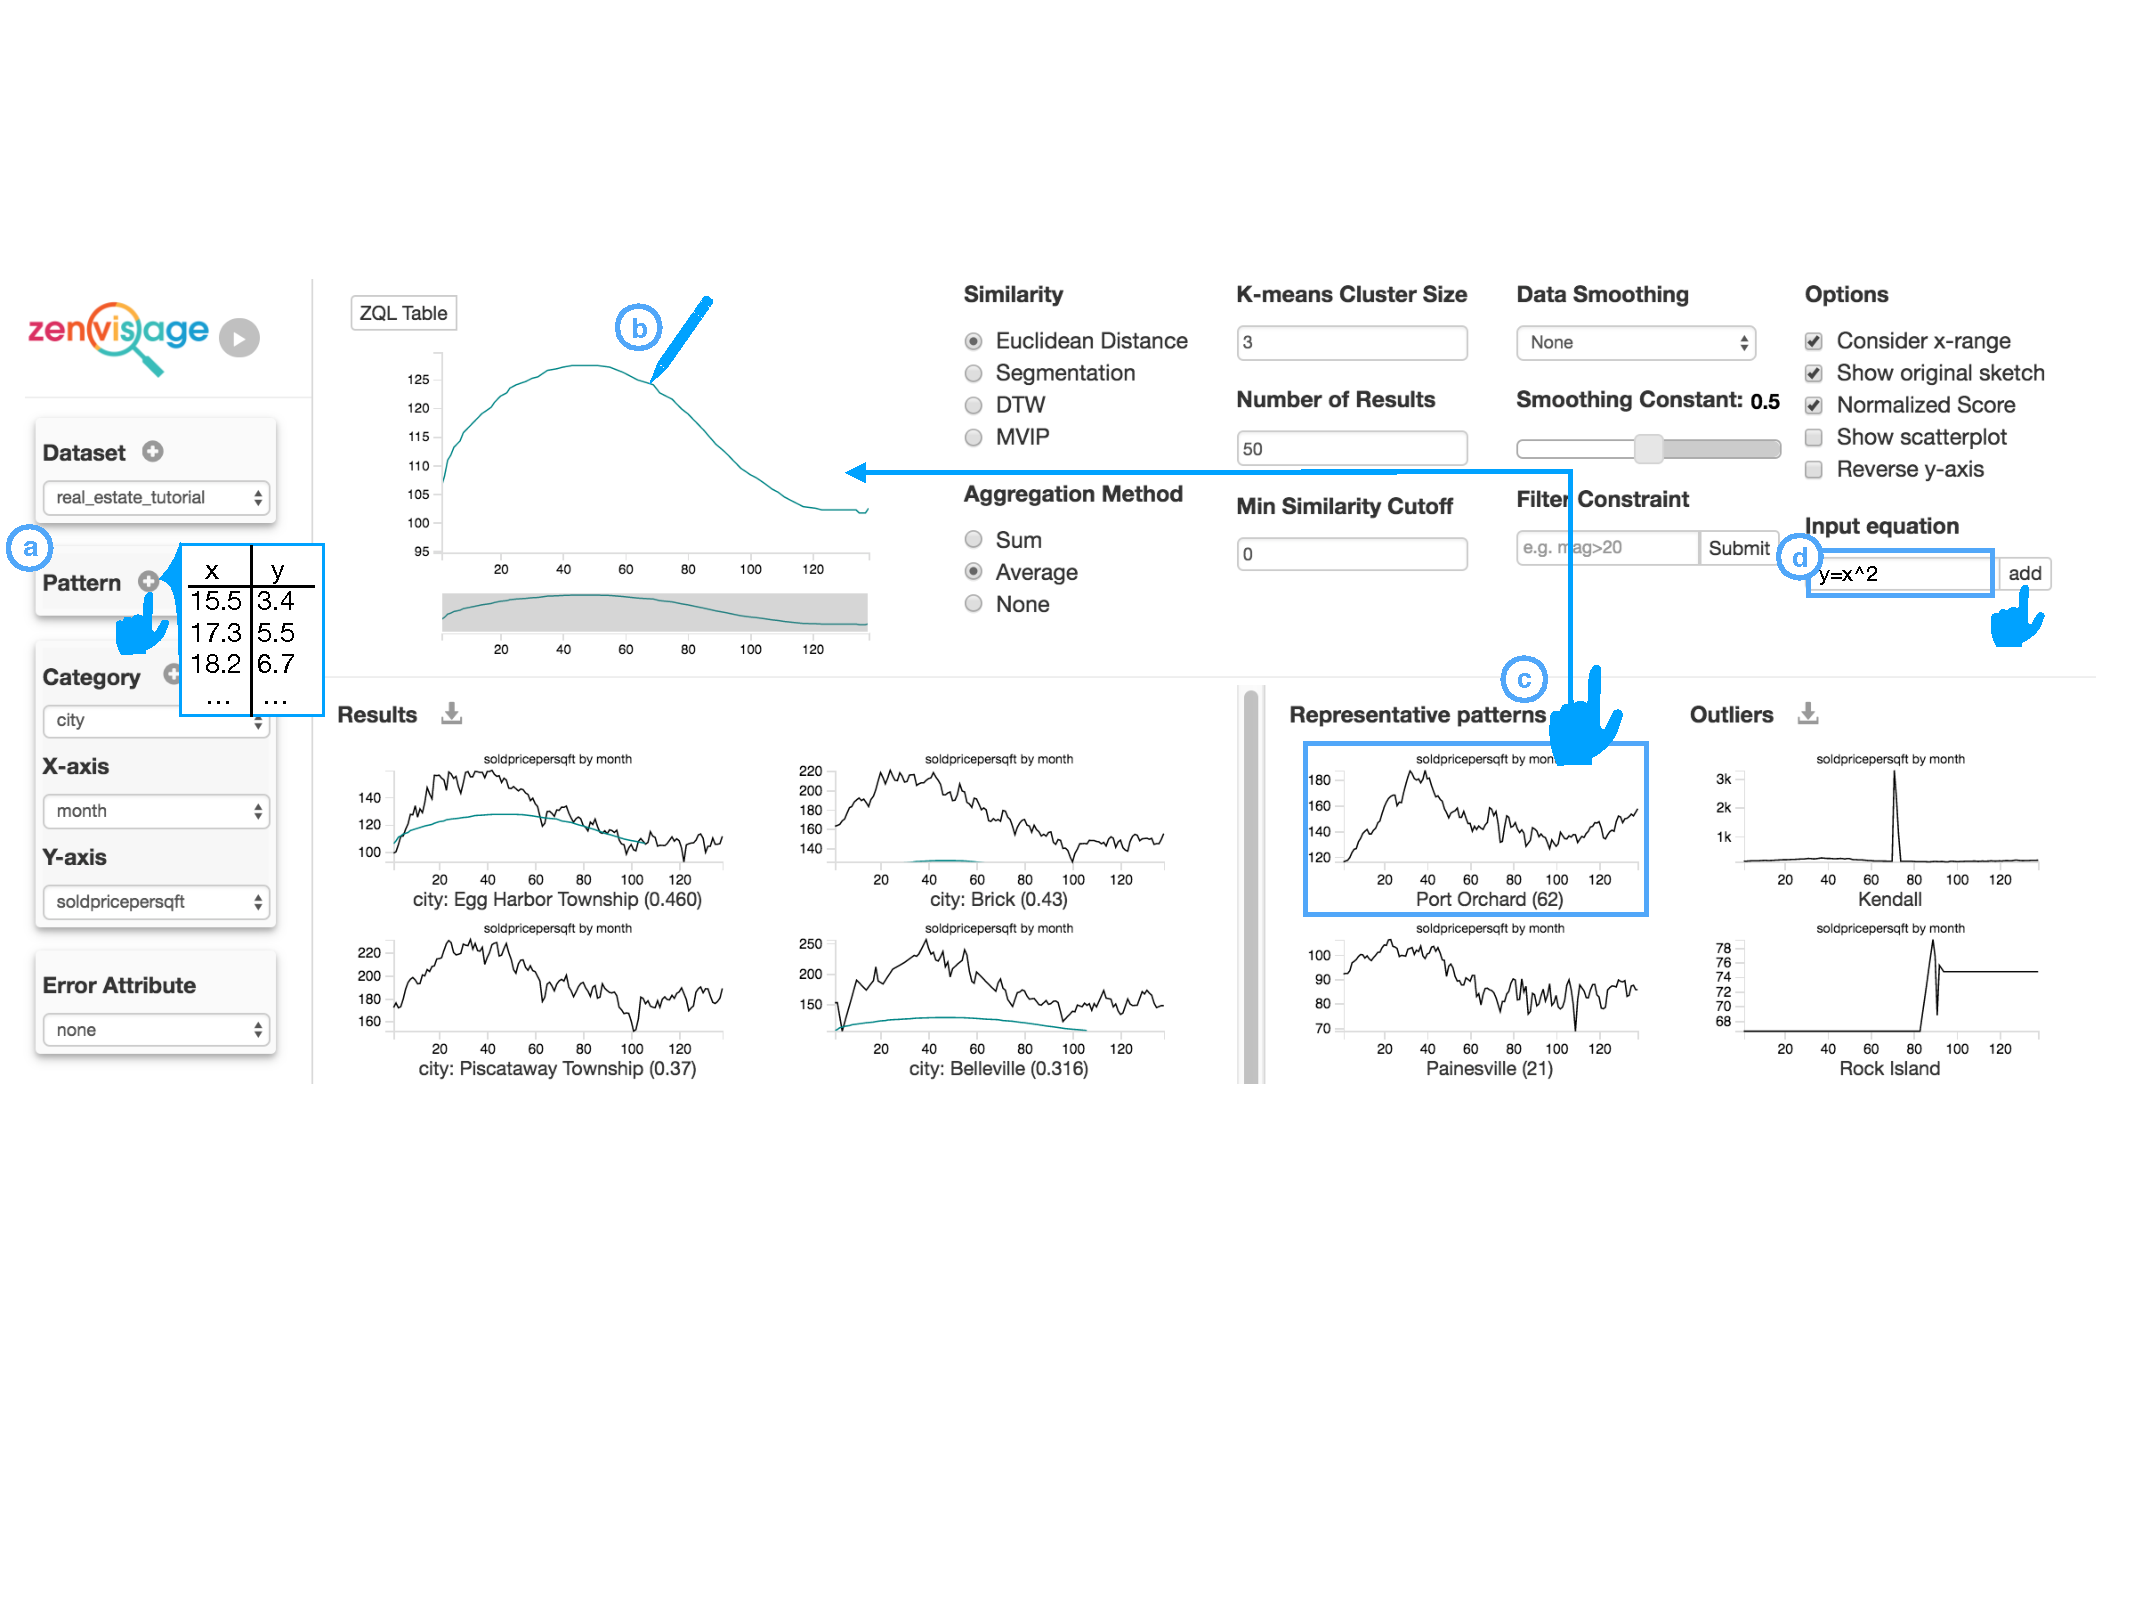
\includegraphics[width=0.8\textwidth]{figures/modalities.pdf}
\caption{\zv offers a variety of querying modalities, including: a) uploading a sample pattern from an external dataset as a query, b) sketching a query pattern, c) dragging-and-dropping an existing pattern from the dataset, and d) inputting an equation as a query.}
\end{figure}

%!TEX root = main.tex
\section{Towards Intelligent Visual Search}\label{sec:vague}
\subsection{The Challenge of Usability-Expressivity Tradeoff}
\par The challenge for supporting vague and complex querying stems from the inevitable design trade-off between query expressivity and interface usability in interactive data exploration systems~\cite{Jagadish2007,Morton2014}. This tradeoff is observed not only in visual data exploration systems, but also true for general ad-hoc data querying. While querying language such as SQL are highly expressive, formulating SQL queries that maps user's high-level intentions to specific query statements is challenging~\cite{Jagadish2007,Khoussainova2010}. As a result, query construction interfaces have been developed to address this issue by enabling direct manipulation of queries through graphical representations~\cite{Abouzied2012}, gestural interaction~\cite{Nandi2013}, and tabular inputs~\cite{Zloof1975,Embley1989}. For example, form-based query builders often consist of highly-usable interfaces that ask users for a specific set of information mapped onto a pre-defined query. However, form-based query builders are often based on query templates with limited expressiveness in their semantic and conceptual coverage, which makes it difficult for expert users to express complex queries. The extensibility of these systems also comes with the high engineering cost, as well as potentially overloading the users with too many potential options to chose from. There is a need for tools that is enables users to formulate rich and complex queries, yet highly usable even for novices.  
%Most systems design exhibits a trade-off between how expressive can the query be and how usable the interface is. 

% \begin{itemize}
% \item Inferring user intent in querying and context is important (both in terms of user input and what is recommended)
% \item tools can not assume user has querying intention. exploration without intention, user don’t know what they are searching for --> Recommendation.
% \item The important thing here is identifying what should be done by the system v.s. requested from user. Inappropriate choice of these will result in lack of expressibility and user feeling lack of control of analysis, limiting exploration.
% \item 
% \end{itemize}
\subsection{Ongoing research and opportunities}
\par Given the tradeoff between expressivity and usability, we can not assume a one-size-fit-all PVQS that could fit the needs for users of different expertise levels and workloads. In this section, we discuss a growing class of systems that accelerates the discovery process of answering an imprecise, fuzzy, and complex queries, with many open research questions including: How can we develop better ways to resolve ambiguity by infering the information needs and intent of analysts? What is the appropriate level of feedback and interactions? How can we develop interpretable visual metaphors that could serve to explain how the query was interpreted and why specific query results are returned to a lay user? We describe three different system challenges in interpreting non-precise queries. Since most visual query systems operates on top of a querying language, we use the linguistical classification scheme to provide an analogy for where the ambiguous aspects of queries may arise during visual data exploration, noting that the use of this analogy by no means limits our analysis to only natural language interfaces.

\begin{figure}[h!]
\centering
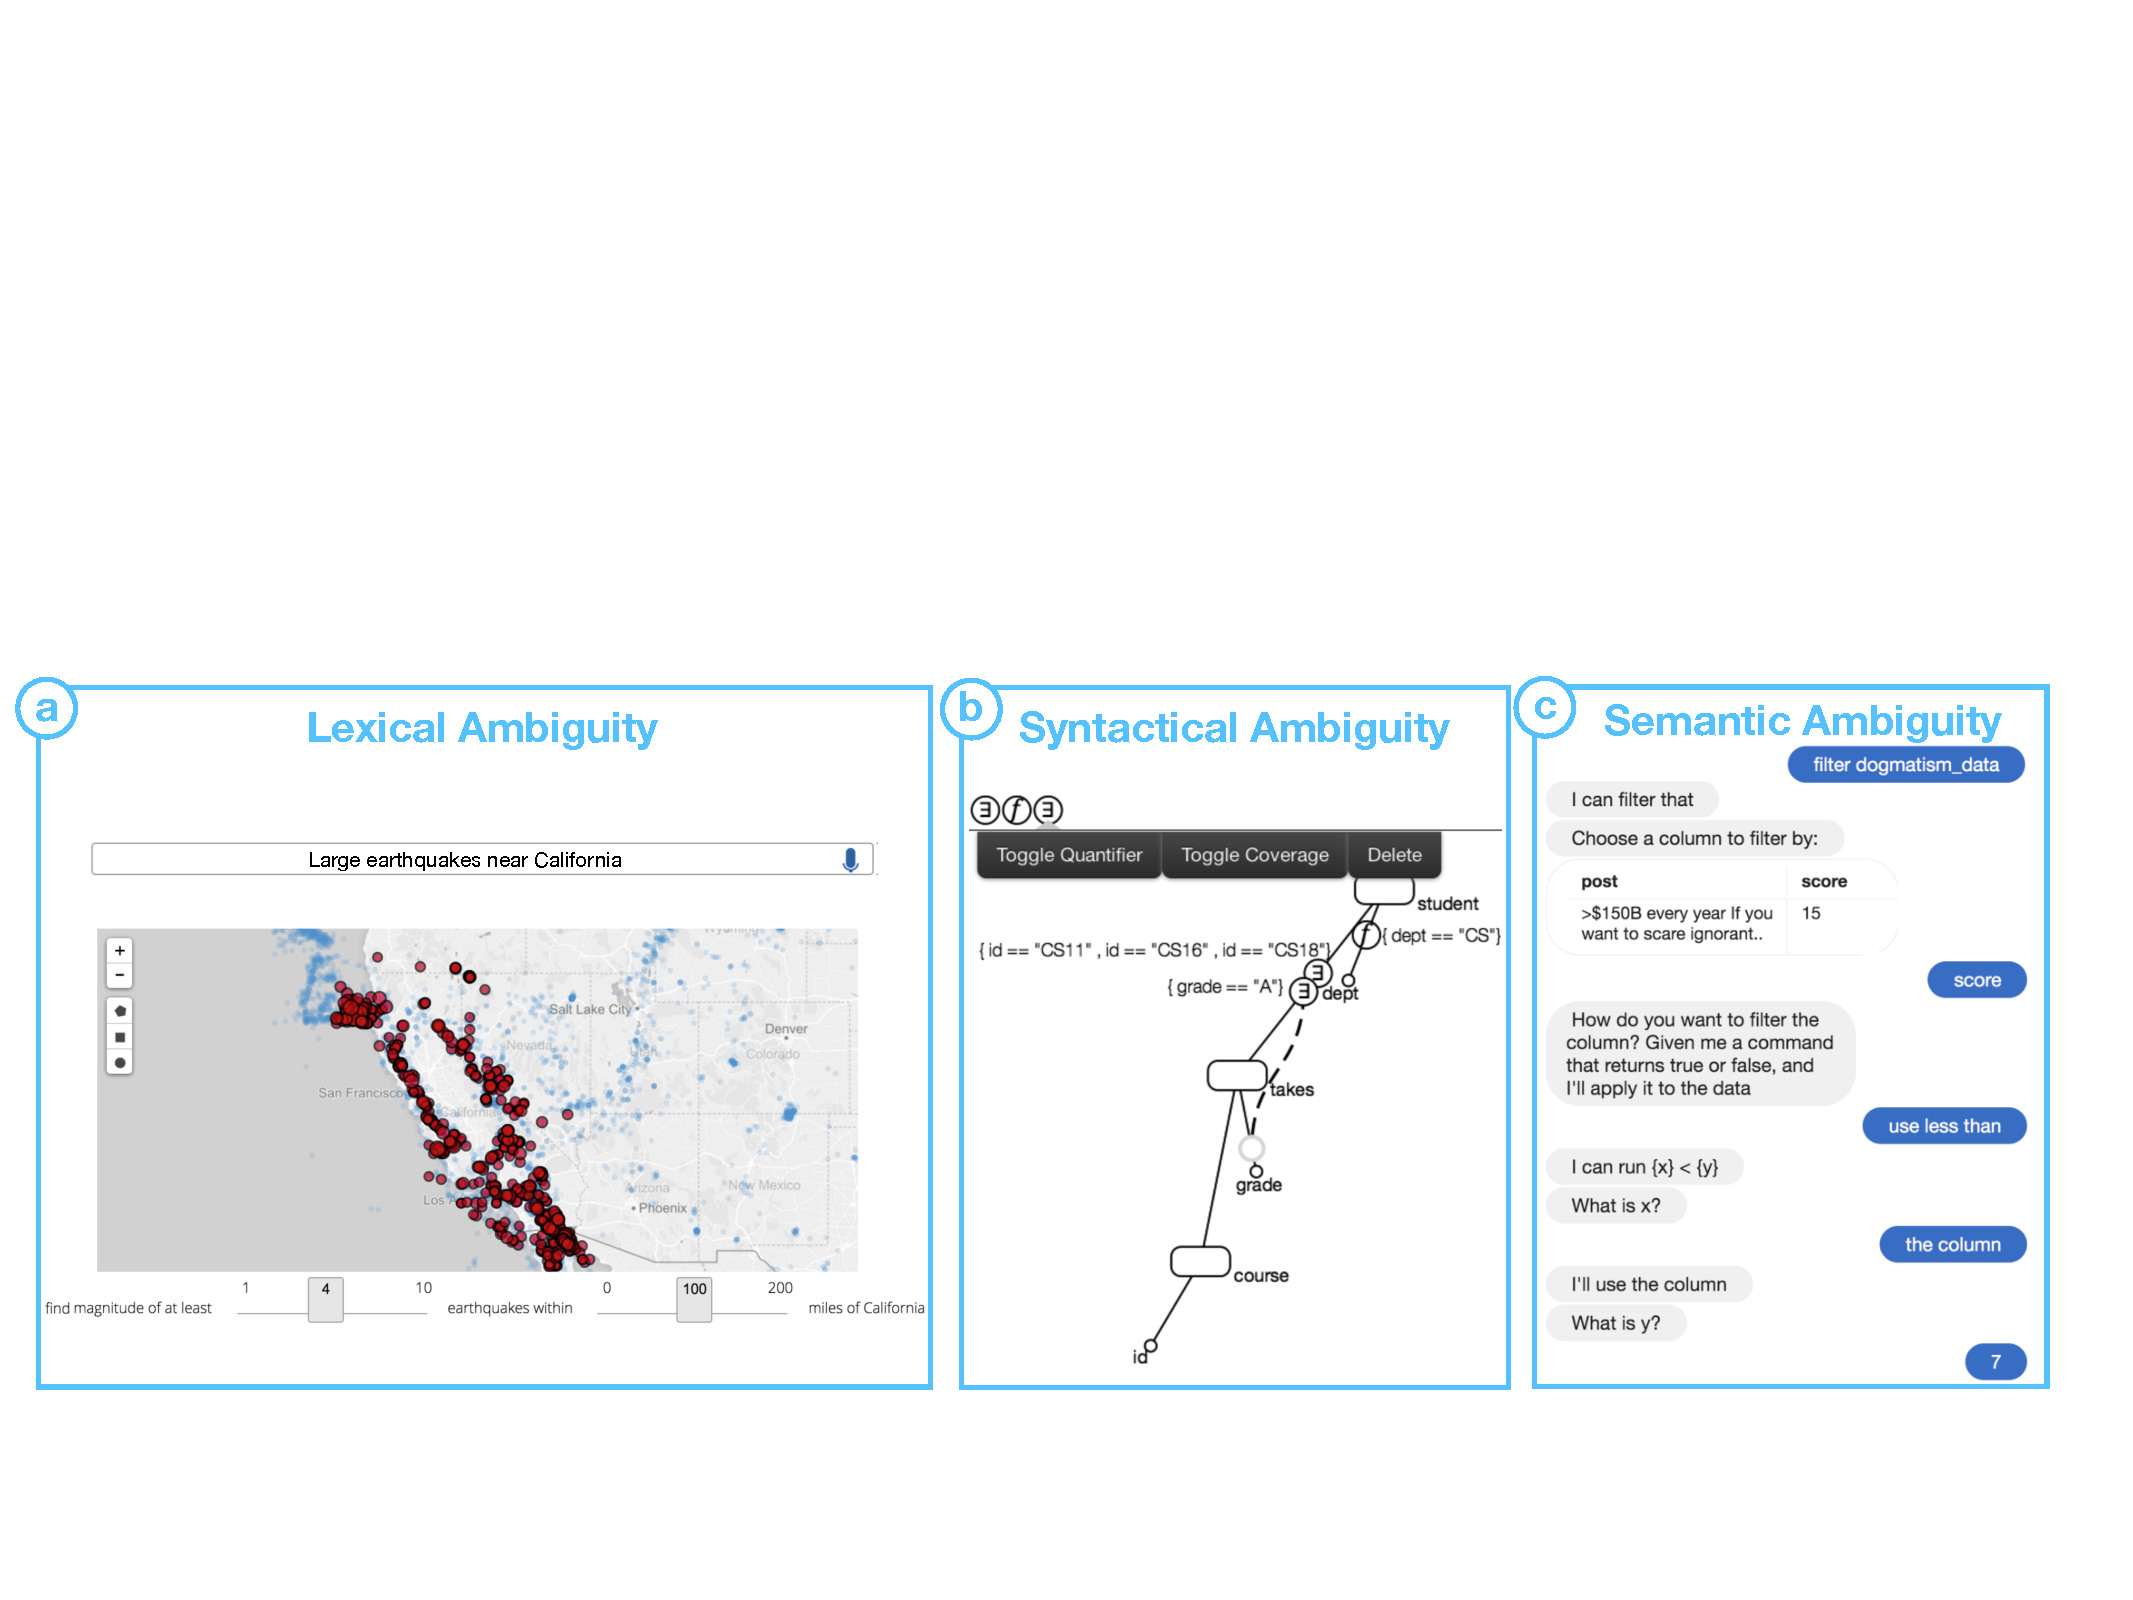
\includegraphics[width=\textwidth]{figures/ambiguity.pdf}
\caption{Examples of fuzzy complex queries: a) Eviza~\cite{Setlur2016} uses ambiguity widgets to enable users to clarify vaguely-defined terms in their input query to resolve lexical ambiguity; b) DataPlay~\cite{Abouzied2012} allow users to toggle between `for all' and `at least one' quantifier to control for syntactical ambiguity; c) Iris~\cite{Fast2018} accepts a vague high-level task description and gather the additional information required through follow-up questions in a nested conversation.}
\label{fig:ambiguity}
\end{figure}
\stitle{Lexical Ambiguity}: Lexical ambiguity involves the use of vague descriptors in the input queries. Resolving these lexical ambiguities has been a subject of research in natural language interfaces for visualization specification, such as DataTone~\cite{Gao2015} and Eviza~\cite{Setlur2016}. These interfaces detect ambiguous quantifiers in the input query (e.g. ``Large earthquakes near California''), and then displays ambiguity widgets in the form of a widget to allow users to specify the definition of `large' in terms of magnitude and the number of miles radius for defining `near', as shown in Figure~\ref{fig:ambiguity}a. These ambiguity widgets not only serve as a way to provide feedback to the system for lexically vague queries, but also is a way for displaying interpretable explanations of how the system is interpreting the input queries. 
%If we consider IVQSs as a layer on top of PVQS (that performs functionalities such as shape-matching, filtering), an IVQS 
% For example,  NaLIR (explanation through query tree, and display multiple interpretations), Eviza (ambiguity widgets), both Eviza/Iris/Ava (follow on clarification utterances). 
Often, there is also ambiguity in the terminology used to describe the query patterns, as we have seen in the \zv user study. We have developed a tool, \ssearch~\cite{Siddiqui2018} that performs efficient  perceptually-aware matching of visualizations using an internal shape query algebra. In the \vida framework, lexical ambiguity is resolved by determining the appropriate \textit{parameters} to \vidaql to achieve the user's desired querying effects.
\stitle{Syntactic Ambiguity}: Syntactic ambiguity is related to the vagueness in specifying how the query should be structured or ordered. For example, DataPlay introduced the idea of syntax non-locality in SQL, in which switching from an existential (at least one) to a universal (for all) quantifier requires major structural changes to the underlying SQL query~\cite{Abouzied2012}. As shown in Figure~\ref{fig:ambiguity}b, DataPlay consist of a visual interface that allowed users to directly manipulate the structure of the query tree in tweaking the query to its desired specification. In the \vida framework, syntactic ambiguities resolution maps portions of the vague queries into to \textit{a series of multi-step workflows} to be executed in \vidaql and expose feedback frameworks to allow users to tweak the query representation directly. %The query modification is done in a declarative manner in that the underlying mechanism in which the visualized workflow gets translated to the querying language is largely hidden from the end-user. 
\stitle{Semantic Ambiguity}: Semantic ambiguity includes addressing `why' questions that are logically difficult to answer, such as `why do these datapoints look different from others?'. For example, Wu and Madden~\cite{Wu2013} have developed Scorpion which traces the provenance of a set of input data tuples to find predicates that explain the outlier behavior. Semantic ambiguity can also arises when the user does not specify their intent completely or explicitly, which is often the case in early stages of visual data exploration. Natural language interface for visual data exploration, such as Evizeon~\cite{Hoque2017} makes use of anaphoric references to fill in incomplete follow-on queries. For example, when a user says `Show me average price by neighborhood', then `by home type', the system interprets the anaphoric reference as continuing the context of the original utterance related to average price on the y-axis. Semantic ambiguity can often be composed of one or more lexical and syntactical ambiguity. For example, in Iris~\cite{Fast2018}, a user can specify a vague, high-level query such as `Create a classifier', then Iris makes use of nested conversations to inquire about what type of classifier to chose and what features to use in the model to fill in the details of the structure and parameters required. If a semantically vague query is not expressible through existing \vidaql, more research may be necessary for developing novel discovery modules in the \vida ecosystem.
%, since the operations involved in the query may not be covered by the limited workflow combinations in the PVQS. 


% Another form of syntactic ambiguity is how  through followup query tweaking 
% nested queries and anaphoric references~\cite{Hoque2017}. Show me relationship between price and -----, then "Break down by -----".
% user intention, composition , Accounting for user interaction, mental models. More global objective taking into account user with the goal of dataset understanding rather than task completion. Need for a unified framework of inference to take all of these into account (e.g. natural language, etc)


%ble to functionalities required to ---- full intent. 

% \stitle{Vague and Ambiguous querying}
 

% \stitle{Recommendation}
% Multimodal visual interfaces, inferring intent from interaction data
% As illustrated in Fig.\ref{system}, these can range from cold-start (no supervision) to input examples, input relations to complete specification.
% \stitle{Complex composition}
% nesting (Ava and Iris)
% In PVQS, the actions are independent of when you do it, when you do them, because they could all be considered as independent series of operations. 

% \par natural language interfaces 
% - joining the flow 
% is a need for an vague or ambiguous specification and global mechanism for ---- nesting ---formulated complex combination. 
%!TEX root = main.tex
\section{Towards Dataset Understanding\label{sec:understanding}}
%general query-free recommendations and continual provenance
\par While our focus in the previous sections have focused on intention-driven queries, where users have some knowledge of what types of questions he may be interested in, one of the key goals of visual data exploration is to promote a better understanding of the dataset to enable users to make actionable decisions. This section discusses systems that helps users become more aware of their dataset and visualize where they are in their analysis workflow. Such systems can often be useful in situations where there is an absence of explicit signals from the user, which can happen when a user is at the beginning of their analysis (commonly known as the `cold-start' problem) or when the user doesn't know what to query for. In this section, we will describe \sbd, a system that provides data summaries and guides users through informative subsets of data, as an example of a system that promotes distribution awareness in a query-free scenario. Then, we will discuss other types of data understanding during dynamic visual data exploration to highlight the challenges and opportunities ahead in this space.
\subsection{\sbd: Promoting Distribution Awareness of Data Subsets with Summary of Visualizations}
%Through Guided ExplorationNavigating Through
%understanding distributions (distribution awareness)
%introduce problem + challenge
\par Common analytics tasks, such as causal inference, feature selection, and outlier detection, require understanding the distributions and patterns present in the visualizations at differing levels of data granularity~\cite{Anand2015,Heer2012,Wu2013}. However, it is often hard to know \textit{what} subset of data contains an insightful distribution to examine. In order to explore different data subsets, an analyst would first have to construct a large number of visualizations corresponding to all possible data subsets, and then navigate through this large space of visualizations to draw meaningful insights. While there are some related work in database literature in constructing informative summaries that help guide users through the complex schema of object-oriented databases\cite{McHugh1997,Yu2006}, these are often focused on table and attribute level information, rather than information about derived from the actual data distributions. The lack of a systematic way to perform these exercises makes the process of manually exploring distributions from all possible data subsets tedious and inefficient~\cite{Sarawagi1998,Sarawagi2000}.
%there is no systematic way to perform these exercises.
% explain what storyboard does
\par To this end, we developed \sbd, an interactive visualization summarization system that automatically selects a set of visualizations to summarize the distributions within a dataset in an informative manner. Figure~\ref{fig:sbd} illustrates an example dashboard generated by \sbd from the Police Stop Dataset \cite{police}, which contains records of police stops that resulted in a warning, ticket, or an arrest. The attributes in the dataset include driver gender, age, race, and the stop time of day, whether a search was conducted, and whether contraband was found. We requested \sbd to generate a dashboard of 9 bar chart visualizations with x-axis as the stop outcome (whether the police stop resulted in a ticket, warning, or arrest/summons) and y-axis as the percentage of police stops that led to this outcome. First, at the top of our dashboard, \sbd highlights three key data subsets that results in a high arrest rate, which looks very different trend than the overall (where the majority of stops results in tickets). Following along the leftmost branch, we learn that even though in general when a search is conducted, the arrest rate is almost as high as ticketing rate, when we look at the Asian population, whether a search is conducted had less influence on the arrest rate and the trend resembles more like the overall distribution.
\begin{figure}[h!]
\centering
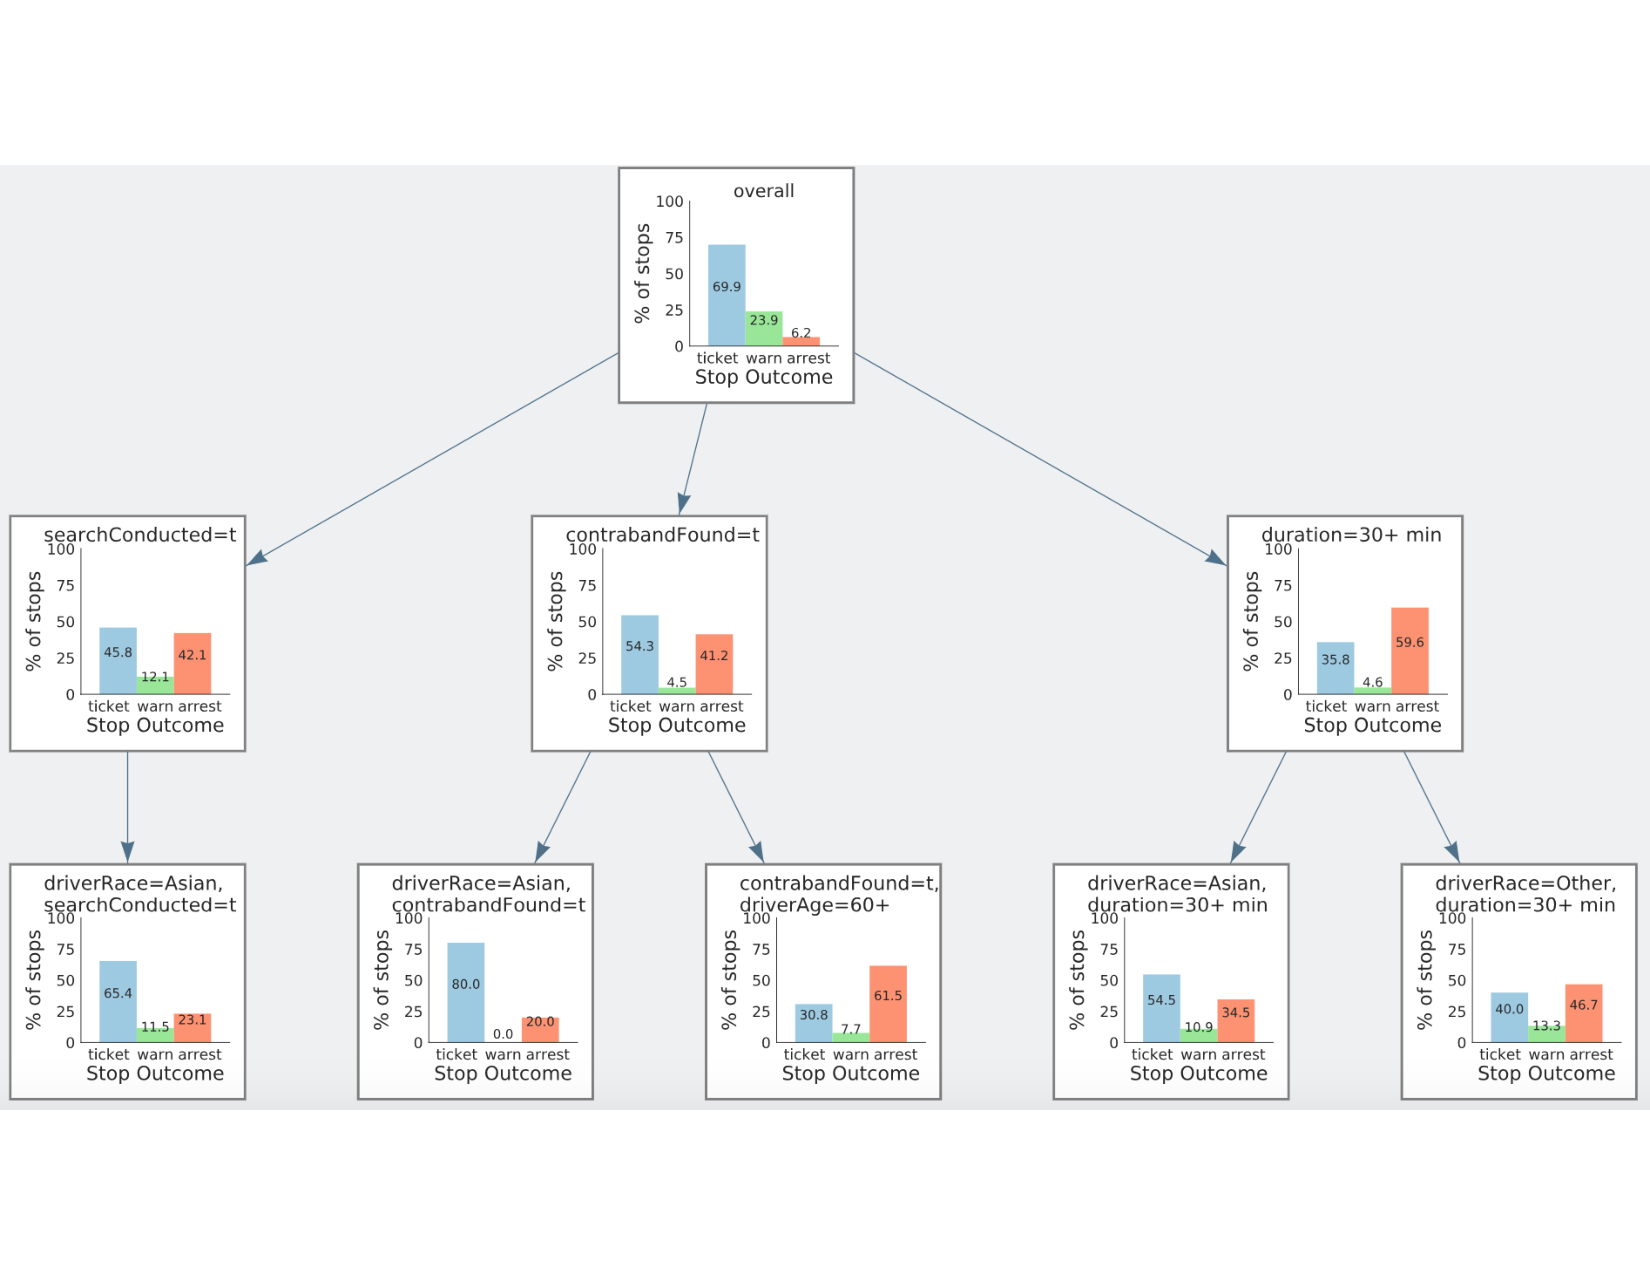
\includegraphics[width=0.7\linewidth]{figures/storyboard.pdf}
\caption{Example dashboard generated by \sbd summarizing the key insights in the Police dataset.}
\label{fig:sbd}
\end{figure} 
% one paragraph on motivation on objectives and explain lattice + traversal 
\par While such summary dashboards are useful for making sense of relationships between data subsets, finding effective visualizations to summarize a dataset is not as trivial as picking individual visualizations that maximizes some statistical measure, such as deviation~\cite{Vartak2015}, coverage~\cite{Sarvghad2017}, or significance testing~\cite{Anand2015}, which can often result in misleading summarizations. The key idea behind our work is understanding how analysts formulate their expectations regarding an unseen visualization in a \textit{data subset lattice}. Applying the idea of data subset lattice from data cube literature~\cite{Harinarayan1996} to filtered bar chart visualizations, we define a visualization as the \textit{parent} of another visualization if the latter visualization can be derived from the first visualization by adding one additional filter constraint. % to organize the relationships between different visualization.
Our formative user study showed that people naturally form their expectations regarding an unseen visualization based on one or more observed parents and that seeing a parent that well describes the unseen visualization leads participants to better estimate the unseen visualization. More importantly, in the absence of an informative parent or in the presence of multiple parents, participants can be misled to form an inaccurate expectation that exhibit higher variance. 
\par Given these insights, the goal of our system is to select \textit{interestingness} and \textit{informativeness} visualizations that can help them make more accurate predictions regarding the unseen visualizations. To model the informativeness of an observed parent in the context of an unseen visualization, we characterize the capability of the parent in predicting the unseen visualization. Our study shows that a visualization is \emph{informative} if its data distribution closely follows the data distribution of the unseen child visualization, since the visualization helps the analyst form an accurate mental picture of what to expect from the unseen visualization. While informative parents contribute to the prediction of an unseen visualization, the most interesting visualizations to recommend are those for which \emph{even the informative parents fail to accurately predict or explain the visualization}. Our problem of constructing the summary dashboard then becomes the problem of finding the k connected visualizations that are most informatively interesting according to this objective. Detailed treatments of our metrics and algorithms can be found in our technical report. \dor{(CITE PLACEHOLDER) Can we put a version of the \sbd paper on arxiv so that we can cite it?}
%explain distribution awareness + its application, its relationship with dataset understnading + how it can be used in other contexts.
\par The effectiveness of \sbd largely comes from how the summary visualizations help analysts become more distributionally aware of the dataset. We define \emph{distribution awareness} as the aspect of data understanding in which analysts make sense of the key distributions across different data subsets and their relationships in the context of the dataset. With distribution awarenes, even though it may be infeasible for an analyst to examine all possible data subsets, the analyst will still be able to draw meaningful insights and establish correlations about related visualizations by generalizing their understanding based on the limited number of visualizations presented in the dashboard. Our evaluation study shows that facilitating distribution awareness through \sbd guides analysts to make better predictions regarding unseen visualizations, ranking attribute importance, and retrieval of interesting visualizations compared to dashboards generated from the baselines. %to make predictions regarding the unseen visualizations
%building future systems that effectively guide analysts towards more meaningful stories for further investigation.
% How ----- is underexplored 
% future research 
% building systems that ---
\subsection{From Distributional to Contextual Awareness: Challenges and Opportunities}
\par The notion of distribution awareness is useful when considering the scenario at one static point in time of the analysis, such as during cold-start. In this section, we introduce a complementary notion of data understanding called \textit{contextual awareness}, which is essential when considering a dynamic analytic workflow for visual data exploration.
 %In this section, we will discuss several other types of data understanding that is essential for effective visual data exploration. Recommendation providing better understanding for overall dataset and understanding. 
\par Contextual awareness is the aspect of data understanding related to the \textit{situation} (what is the information that I'm currently looking and how did it come about?) and \textit{provenance} (what have I explored in the past and where should I look next?) of data. Situational understanding involves recognizing what data is in the current scope of analysis, including making sense of the data attributes and schema and keeping track of what filter or transformations have been applied to the displayed data. Provenance understanding is associated with the analyst's past analysis actions on the data. As an example, an analyst may be interested in how the sales price of a product changes as a function of other dimensions variables, such as geographic location, year sold, and product type. Situation information informs him that he is looking at a bar chart with \textsc{x=TYPE}, \textsc{y=AVG(PRICE)}, whereas provenance information points to the fact that he should explore the geographic dimension, since he has already explored the temporal attribute \textsc{YEAR}.
\par Within a dataset, provenance is essential in helping users navigate through the space of possible analysis actions and provide users with sense of coverage and completion. While the problem of data provenance has been well studied in database literature~\cite{Buneman2006,Cui2003,Woodruff1997}, the effects of showing provenance information to users during data analysis is an important but underexplored area. The notion of adding navigational cues to guide exploration in visual information spaces was first proposed in Willet et al.'s work on \textit{scented widgets}~\cite{Willett2007}. In Pirolli and Card's theory of information foraging, scents are cues that signifies the percieved benefit that one would recieve during a search. Scented widgets adds to existing search interfaces by embedding visualizations that provide informational scents, such as histogram distributions of how popular a particular value is among users or using color to encode the size of a dataset in a drop-down menu. Recently, Sarvghad et al. have extended the idea of scented widgets to incorporate dimension coverage information during data exploration, including which dimensions have been explored so far, in what frequency, and in which combinations~\cite{Sarvghad2017}. Their study shows that visualizing dimension coverage leads to increased number of questions formulated, findings, and broader exploration. Interpretable and non-disruptive cues that enables users to visualization provenance history helps sustain contextual awareness and guides users towards more informative next steps in their analysis.%than participants who had no access to coverage information
\par Mechanisms that facilitate distribution awareness for users can effectively couple with contextual awareness in dynamic exploration situations to help update the user's mental model on the current data context. For example, the representative and outlier patterns in \zv provides summaries of data in context. When a dataset is filtered, the representative trends are updated accordingly. By being aware of both the context and the distributions, the users becomes distributionally aware of how the typical patterns and trends of the distributions changes in a particular context. %(i.e. I'm only looking at data filtered with ....),an overview of typical trends for the data to be queried.
\par While our discussion above have been focused on how to design systems that can help facilitate these aspects of user's awareness in dataset understanding, these ideas can be generalized to principles in designing IVQS discussed in Section~\ref{sec:vague}. An IVQS needs to be distributionally and contextually aware, by make use of information about the data (distribution awareness), the analytic context, and situation jointly in making timely recommendations. In other words, these systems should not only facilitate these aspects of data awareness, but also need to make use of this information to make recommendations that can guide analysts towards meaningful stories and insights for further investigation.
%For example, contextual awareness can inform the system that the user's current situation (x,y, encoding, etc.), while a distributionally aware system may recommend a highly-skewed data subset as interesting, a situational aware system may realize a variable have been explored extensively in the past and recommends it accordingly. 

% inference and descisions intepretable.
% , rather than the system's awareness of the user's context, situation ,etc. Ideally, an intelligent system  should 
% related works have focussed on making specification easier, but not really trying to understnad user intent or what might the user want to see.

%!TEX root = main.tex
\section{Concluding Remarks\label{sec:conclusion}}
\par Data is inherently agnostic to the diverse information needs any user may have. Visual data exploration systems help bridge the gap between what users want to get from the data through querying and what insights the data has to offer through recommendations. To more facilitate a more productive collaboration, in this paper, we discuss how precise visual query systems provide informative visualizations to accelerate the process of data discovery, how intelligent visual query systems account for vague and complex query through query refinement feedback, and how recommendations could promote better distributional and contextual awareness for users. We hope that the agenda sketched out in this paper sheds light to the many more exciting research questions and opportunities to come in this nascent growing field.% and encourage database researchers to ----- tackle in this space.
% This paper discusses how to better support these and how ----. Section~\ref{sec:precise} discusses how precise visual query systems provide informative visualizations to accelerate the process of data discovery. Section~\ref{sec:vague} discusses mixed-intiative systems that accounts for vague and complex query and allow users to provide feedback to refine their queries. Section \ref{sec:understanding} discusses the challenges and opportunities in moving from intention-driven querying to facilitating more integrated data understanding and awareness during the analysis workflow.

% Data is agnostic to the user, intention ---, by building tools---, Section \ref{sec:precise} to \ref{sec:vague} have focussed on extracting what user want from data. bridging together what user want from data, what data has to offer, supporting interactive discourse between the two. 

% \par In this paper, we advocate supporting a desiderata consisting of  3`I's in the cycle of visual data exploration:
% \begin{itemize}
% 	\item \textbf{Informative}: Section~\ref{sec:precise} discusses how precise visual query systems provide informative visualizations to accelerate the process of data discovery. 
% 	\item \textbf{Iterative}: Section~\ref{sec:vague} discusses mixed-intiative systems that accounts for vague and complex query and allow users to provide feedback to refine their 
% 	Joining the flow, query refinement, dialogue (not a one-shot query), feedback and recommendation, expressivity (how easy is it to express what to do via interactions) and diversity of actions that could be performed.
% 	\item \textbf{Integrated}: Section \ref{sec:understanding} discusses the challenges and opportunities in moving from intention-driven querying to facilitating more integrated data understanding and awareness during the analysis workflow.
% \end{itemize}

%  Either using one-size-fits-all statistics, templates, heuristics as a solution or problem only applicable to a subset of analytic tasks\cite{Vartak2015,Vartak2017}. 

\section*{Acknowledgement}
A. P. acknowledges support from grants IIS-1513407 and IIS-1633755 awarded by the National Science Foundation, grant 1U54GM114838 awarded by NIGMS and 3U54EB020406-02S1 awarded by NIBIB through funds provided by the trans-NIH Big Data to Knowledge (BD2K) initiative (www.bd2k.nih.gov), and funds from Adobe, Google, and the Siebel Energy Institute. The content is solely the responsibility of the
authors and does not necessarily represent the official views of the funding agencies and organizations. \dor{copied this from the crowdsourcing vision paper, might have to change grant number and sources accrodingly. Might also want to include acknowledgement for collaborators here too.}
{\footnotesize \bibliographystyle{named}
\bibliography{reference}}
\end{document}
